\chapter{Ingeniería de software}
\label{sec:sftw}
Todo el desarrollo de este trabajo se ha realizado en Python. Python es un lenguaje de programación de alto nivel diseñado por Guido van Rossum y aparece en 1991. Este lenguaje está centrado en la legibilidad del código, siendo un lenguaje interpretado. \linebreak
Python también provee un gestor de paquetes llamado \textit{pip} que permite crear e instalar librerías externas, proporcionando así una mayor comodidad para hacer uso de librerías externas que lenguajes como C no tienen. \\
\linebreak
Uno de los mayores inconvenientes que tiene Python es que es un \textit{lenguaje interpretado} donde un interprete lee y ejecuta las instrucciones escritas en un \textit{script}, haciendo que el rendimiento sea menor que el de un programa que haya sido compilado.\\
\linebreak
\section{Biblioteca usadas}
Para realizar este trabajo, se ha hecho uso de una serie de \textbf{bibliotecas externas} que incrementan las capacidades ofrecidas por el lenguaje de manera nativa, ya que la gran mayoría de herramientas que han sido usadas no vienen instaladas por defecto.\\
A continuación, se listan las librerías usadas y una breve descripción de las herramientas/características que ofrecen:
\begin{itemize}
    \item \textbf{scikit-learn:} Es una biblioteca para aprendizaje automático que incluye una gran cantidad de algoritmos (SVM, árboles de decisión, Random Forest, etc) y distintas utilidades (métricas, validación cruzada, división de conjunto de entrenamiento y de test, etc). Es de software libre y está programada en C, C++ y Python.
    \item \textbf{Numpy}: Es una biblioteca que da soporte para crear vectores y matrices de grandes dimensiones junto con una colección de funciones para operar con estos tipos de datos. De nuevo, es una biblioteca de software libre y está escrita en Python, C y Fortran.
    \item \textbf{matplotlib}: Es una biblioteca para generar gráficos escrita en C++ y Python.
     \item \textbf{seaborn}: Es una biblioteca basada en \textit{matplotlib} que proporciona una interfaz de alto nivel para crear gráficos. Está escrita en Python.
     \item \textbf{pandas}: Es una biblioteca para la manipulación y análisis de datos.  Está escrita como una extensión de \textit{numpy}, siendo también software libre.
     \item \textbf{xgboost}: Biblioteca que proporciona una implementación para el algoritmo XGBoost.
\end{itemize}
Para facilitar la instalación de todas estas librerías de manera que no proporcionen conflictos, se ha optado por usar \textit{pip}.
\section{Entorno de programación}
Para evitar conflictos e instalar las librerías usada de forma aislada a las librerías de sistema, se ha echo uso de \textbf{entornos virtuales} de Python. La principal ventaja de hacer uso de estos entornos virtuales es que aíslan todas las librerías del resto de librerías instaladas, evitando así conflictos con las del sistema o incluso conflictos entre librerías necesarias para varios proyectos.
\section{Paquete de software desarrollado}
Además del uso de estos entornos virtuales, se ha creado un \textbf{paquete} con distintas utilidades que se han desarrollado, facilitando así la re-utilización de código y el mantenimiento del mismo, ya que \textit{pip} permite gestionar automáticamente las dependencias indicadas en el archivo de configuración y facilitando la instalación correcta de las distintas utilidades desarrolladas.
A continuación se va a mostrar un diagrama de paquetes para explicar como se ha estructurado el paquete:
\begin{figure}[H]
    \centering
    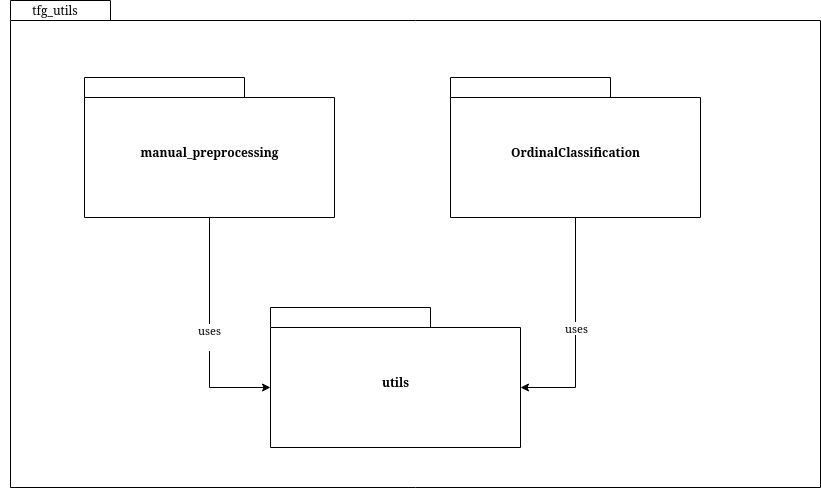
\includegraphics[scale=0.5]{diagrama_paquetes_tfg}
    \caption{Diagrama para paquete \textbf{tfg\_utils}}
    \label{dig:paquetes_tfg}
\end{figure}
\begin{itemize}
    \item \textbf{manual\_preprocessing} contiene una serie de funciones usadas en la fase de pre-procesamiento.
    \item \textbf{OrdinalClassification} contiene un paquete con la implementación del algoritmo de clasificación ordinal explicado en \ref{sec:ord}-\nameref{sec:ord}.
    \item \textbf{utils} contiene una serie de funciones que se han usado para todos los scripts. Contiene funciones para calcular las métricas, hacer la validación cruzada, etc.
\end{itemize}
\subsection{Paquete para clasificación ordinal}
 A continuación se va a mostrar un diagrama explicando las clases que contiene el paquete \textbf{OrdinalClassification}:
 \begin{figure}[H]
     \centering
     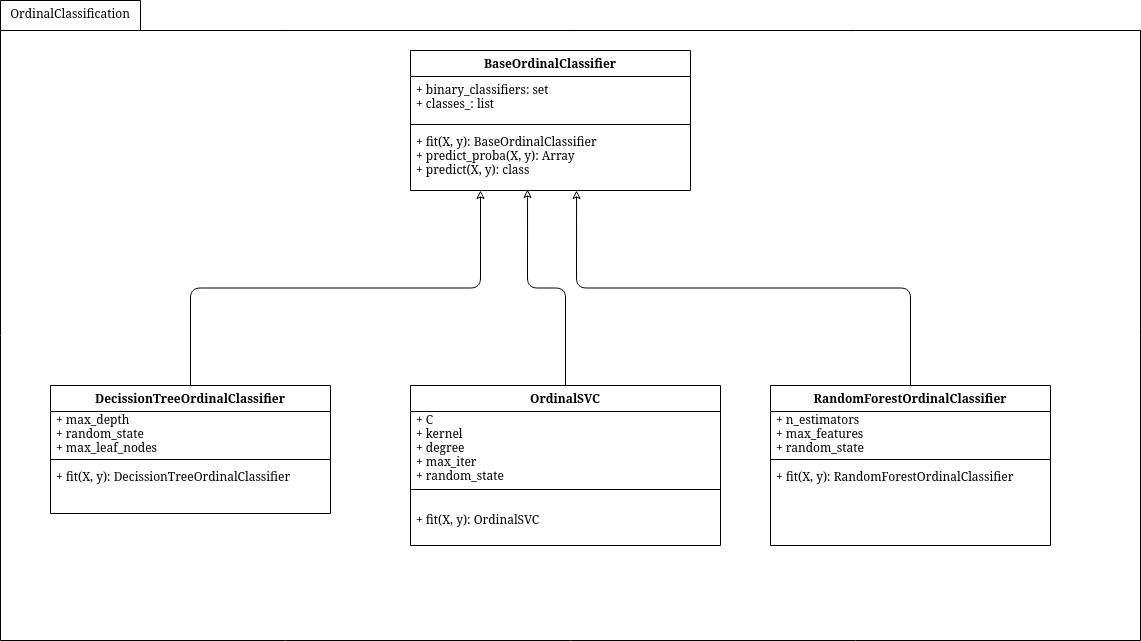
\includegraphics[scale=0.35]{diagrama_od}
     \caption{Diagrama para paquete \textbf{OrdinalClassification}}
     \label{dig:paquetes_od}
 \end{figure}
Las funciones \textbf{\textit{predict}} (predice una clase dada una entrada) y \textbf{\textit{predict\_proba}} (dada una entrada predice la probabilidad de que una muestra pertenezca a cada clase)  son iguales para todos los modelos, se ha optado por crear una clase abstracta que va a implementar estas funciones. El resto de clases implementará el método \textbf{\textit{fit}} con el modelo seleccionado. \\
Cabe destacar que la implementación de estos modelos es compatible con todas las utilidades que proporciona \textit{scikit-learn}, facilitando mucho el proceso de validación cruzada, optimización de parámetros, etc.\\
\subsection{Paquete para clasificación multi-etiqueta simple}
\label{sec:sftw-mlc}
\section{Scripts}
Finalmente, la carpeta \textbf{\textit{scripts}} contiene todos los scripts usados para entrenar y mostrar resultados. Estos scripts son capaces de guardar la información obtenida en formato JSON y guardarlos en disco, facilitando así la integración con otras aplicaciones.\\
\linebreak
Se ha añadido también un script para comparar los resultados obtenidos por dos o más modelos, generando las gráficas que se han mostrado en secciones anteriores. Este script obtiene la información en formato JSON, especificando la ruta al archivo por linea de comandos. \\
\linebreak
Todos estos scripts, si se ejecutan con la opción \textbf{\textit{-h}} se mostrará una ayuda con todos los parámetros aceptados y una explicación de cada uno de ellos.
\section{Instalación del software}
Para instalar el software se necesita una versión 3.x de Python (durante el desarrollo se ha usado la versión 3.9.6) y el gestor de paquetes \textbf{pip}. Una vez descargado el repositorio(https://github.com/antoniomanuelfr/TFG.git), simplemente ejecutando el comando \textit{pip3 install .} en la carpeta padre del repositorio, se instalará el paquete junto con todas las dependencias.
A continuación se muestra una captura de pantalla del proceso completo para ejecutar el algoritmo \nameref{alg:knn}:
 \begin{figure}[H]
    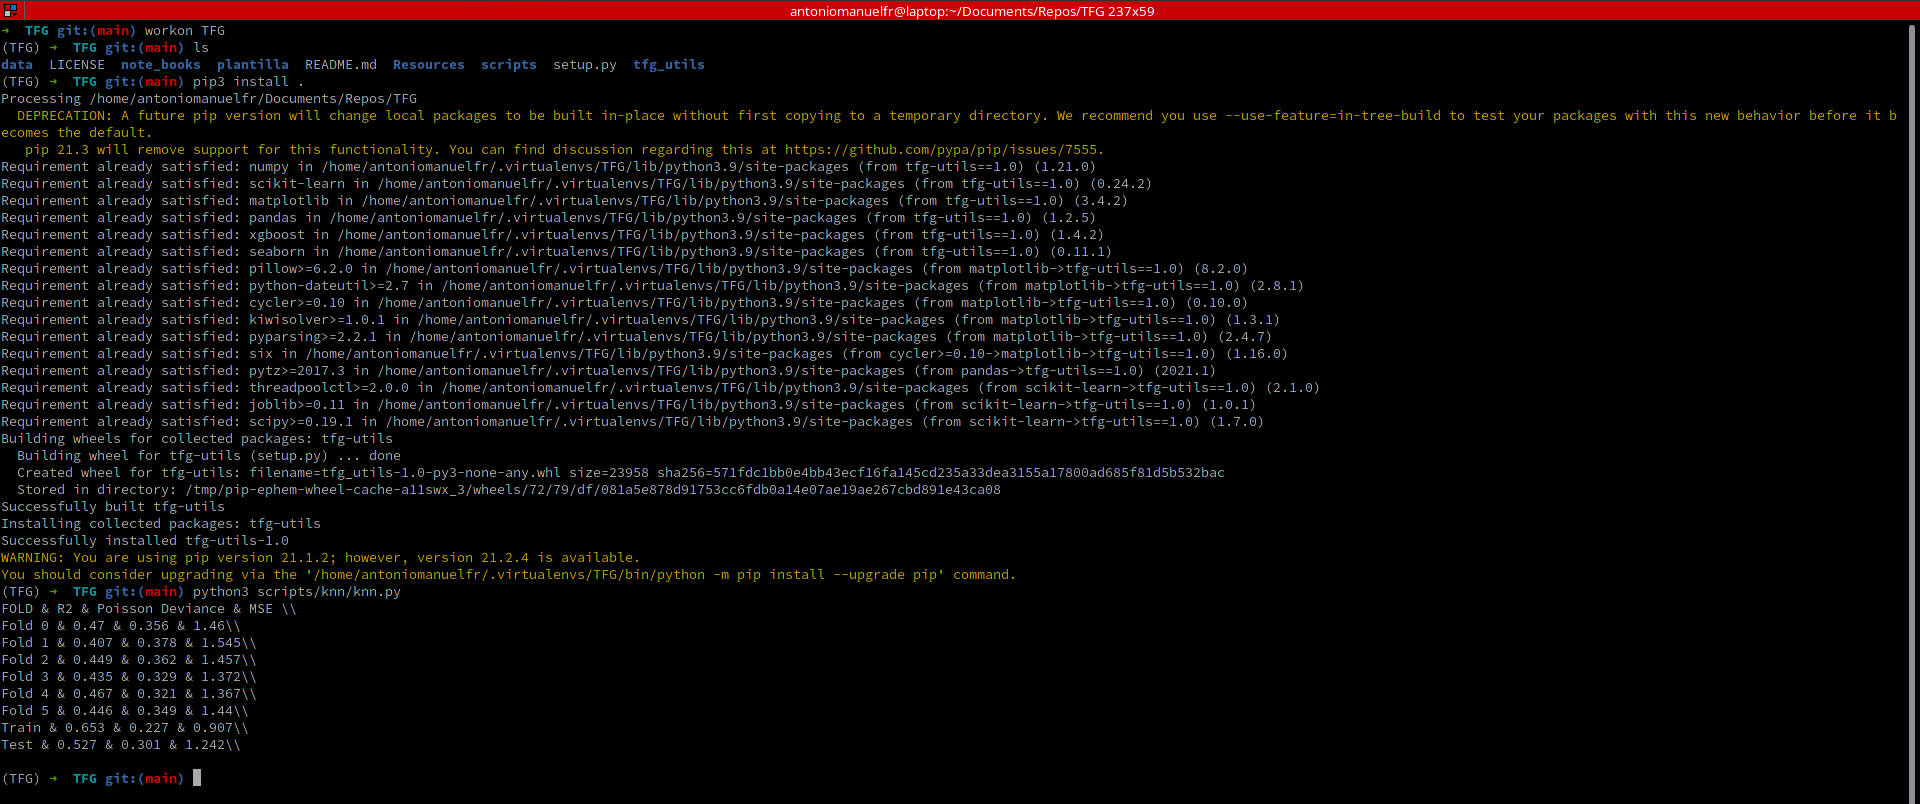
\includegraphics[scale=0.3]{ejemplo_ex}
    \caption{Ejemplo de ejecución completa para KNN}
    \label{cap:ex}
\end{figure}